\documentclass[11pt]{beamer}
\usetheme{Warsaw}
\usecolortheme{default}
\usepackage[utf8]{inputenc}
\usepackage[english]{babel}
\usepackage{multicol}
\usepackage{ragged2e}
\usepackage{graphicx,url,hyperref,doi}
\usepackage{tikz}
\usepackage{adjustbox}
\usepackage{multicol}

\usepackage[numbers, sort, compress]{natbib}
\bibliographystyle{unsrtnat}

\begin{document}
 
\title[Defensa de Tesis  \hspace{35mm} \insertframenumber/\inserttotalframenumber]{Sentiment Analysis through Conversational Data}
\institute{\\Universidad Autónoma de Nuevo León \\Facultad de Ingeniería Mecánica y Eléctrica}
\author{Alexander Espronceda Gómez \\ Ing. en Tecnologías de Software}
\date{\today}

\logo{FIME UANL}

\frame{\titlepage}

\begin{frame}{Índice}
\transdissolve
\begin{center}
\begin{multicols}{2}
  \footnotesize{\tableofcontents}	
\end{multicols}
\end{center}
\end{frame}

\begin{frame}
  \begin{abstract}
    In this thesis, open-sourced software is proposed, which interprets the text entered by a person and determines how they are feeling at the moment, with the purpose of being used in tandem with another software or algorithms focused on conversational data.
  \end{abstract}
\end{frame}

\section{Introduction}

\begin{frame}{Introduction}
  \begin{figure}[!h]
	\centering
	\includegraphics[scale=0.15]{BrainMap}
	\label{fig:brainmap}
	\caption{Lateral brain map of the parts in charge of the empathy processes. Drawing generated using BrainPainter \citep{img1}.}
	\end{figure}
\end{frame}

\subsection{Justification}
\begin{frame}{Justification}
  \begin{block}{Justification}
  This project could prove especially useful towards being used in projects designed for people who have trouble discerning when to console someone or having an idea of how other people or even themselves feel.
To this end, the decision was made to work on this project.
  \end{block}
\end{frame}

\subsection{Hypothesis}
\begin{frame}{Hypothesis}
  \begin{block}{Hypothesis}
  Using supervised machine learning with a neural network could accurately classify the sentiment behind an input text as ``Good'', ``Neutral'' or ``Bad'', with the purpose of being implemented in tandem with another software or algorithms focused on conversational data.
  \end{block}
\end{frame}

\subsection{Objective}
\begin{frame}{Objective}
  \begin{block}{Objective}
  Make software capable of determining how the person that writes the input text is feeling according to the words in it, while keeping the code open-source so it can be used in other projects. This could be achieved thanks to the technology present in machine learning algorithms and an extensive amount of datasets.
  \end{block}
\end{frame}

\section{Background}

\subsection{Basic Concepts}
\begin{frame}{Basic Concepts}
	\begin{description}
	\item[Machine Learning]{Also known as ML. The type of algorithm needed for automatic processing, making the machine ``learn'' (hence the name) over time given enough data.}
	\item[Neural Network]{A Machine Learning algorithm that uses weights and filters to output data.}
	\item[Natural Language Processing]{This is the method used for the algorithm to understand the content of the sentences, this is usually achieved by using tokenization but a preset corpus can also be used.}	
	\end{description}
\end{frame}

\begin{frame}{Basic Concepts}
	\begin{description}
	\item[Sentiment Analysis]{This involves a ML algorithm, usually a Neural Network, that is able to analyze sentences and classify them according to the words used.}
	\item[Corpus]{Preset internal dictionary that the algorithm uses.}
	\item[Tokenizing]{Process that converts every word in the lexicon to an assigned number for easier 	processing}
	\end{description}
\end{frame}

\subsection{Supervised Machine Learning}
\begin{frame}{Concept}
Supervised ML can be described, broadly and figuratively speaking, as a black box where some data is inserted as an input and numbers come out of it as an output \citep{rf8}. 

This output, as opposed to other types of Machine Learning, is later analyzed and compared to real life data.
\end{frame}
\begin{frame}{Machine Learning Stages}
	\begin{block}{Training}
		\begin{itemize}
		 \item Processes the inputs and makes educated guesses.
		 \item Changes weights accordingly.
		\end{itemize}
	\end{block}
	\begin{block}{Validation}
	Input is fed to the algorithm and information needs to be compared to the real results to test the accuracy percentage.
	\end{block}
\end{frame}

\subsection{Sentiment Analysis}
\begin{frame}{Concept}
	\begin{block}{Process}
		\begin{itemize}
		\item The sentence to analyze is broken down to its component parts, this process is called \textit{tokenization}, and the resulting products are called \textit{tokens}.
		\item Every token is then tagged, making it part of an internal dictionary or \textit{lexicon}
		\item A score is assigned to every token depending on the used dataset.
		\end{itemize}
	\end{block}
\end{frame}

\subsection{Tokenization}
\begin{frame}{Tokenization Example}
	\begin{center}
	\fbox{This is an example text}\\
	\vspace*{2cm}
	We can tell there are 5 words in the example phrase. So:\\
	\fbox{1,	2,	3,	4,	5}
	\end{center}
\end{frame}
\begin{frame}{Tokenization Example}
	\begin{center}
	\fbox{This is another example}\\
	\vspace*{2cm}
	If we used the same tokenizer:\\
	\fbox{1,	2,	6,	4}
	\end{center}
\end{frame}

\section{Related Work}
\begin{frame}{Related Work}
	\begin{table}[!h]
	\caption[Comparison between existing literature and the present work.]{Comparison between existing literature and the present work: \checkmark indicates the fulfillment of a criterion, otherwise $\times$ is used.}
	\vspace{0.5cm}
	\centering
	\begin{adjustbox}{width=1\textwidth}
	\begin{tabular}[t]{lccccc}
	\hline
		\textbf{Project} & \textbf{Neural Network} & \textbf{Text Processing} & \textbf{Sentiment Analysis } & \textbf{Open Source} & \textbf{Modular}
	\\ \hline
	\citet{rf10} Maximum Entropy & \checkmark & \checkmark & \checkmark & $\times$ & $\times$
	\\ \hline
	\citet{rf10} Support Vector Machines & \checkmark & \checkmark & \checkmark & $\times$ & $\times$
	\\ \hline
	\citet{rf10} Lingpipe & \checkmark & \checkmark & \checkmark &  $\times$ & $\times$
	\\ \hline
	\citet{rf6} & \checkmark & \checkmark & \checkmark &  $\times$ & $\times$
	\\ \hline
	\citet{rf14} & \checkmark & \checkmark & $\times$ & \checkmark & $\times$
	\\ \hline
	\citet{rf5} & \checkmark & \checkmark & \checkmark & \checkmark & $\times$
	\\ \hline
	\citet{rf11} & \checkmark & \checkmark & $\times$ &  \checkmark & $\times$
	\\ \hline
	\citet{rf12} & \checkmark & \checkmark & \checkmark &  \checkmark & $\times$
	\\ \hline
	\citet{rf13} & \checkmark & \checkmark & \checkmark & $\times$ & $\times$
	\\ \hline
	\citet{rf15} & \checkmark & \checkmark & $\times$ &  \checkmark & $\times$
	\\ \hline
	\citet{rf16} & \checkmark & \checkmark & \checkmark & \checkmark & $\times$
	\\ \hline
	The present work & \checkmark & \checkmark & \checkmark & \checkmark & \checkmark
	\\ \hline
	\end{tabular}
	\end{adjustbox}
	\end{table}
\end{frame}

\section{Proposed Solution}
\begin{frame}{Tools}
	\begin{block}{Tools}
		This project is built on Python v3.8.10, The libraries used for this project to come to fruition are TensorFlow v2.6.0 and Keras v2.6.0 for the Neural Network section and Natural Language Toolkit v3.5 (also known as NLTK) for the tokenization and stemming process.
	\end{block}
\end{frame}
\begin{frame}
	\begin{multicols}{2} 
		\begin{figure}[!h]
		\centering
		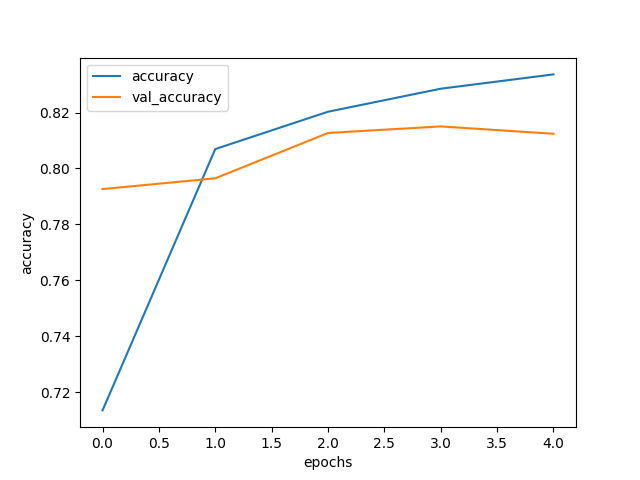
\includegraphics[scale=.35]{Accuracy_Exp9}
		\label{fig:AccExp9}
		\caption{Accuracy values of the finished 	project}
		\end{figure}
		\begin{figure}[!h]
		\centering
		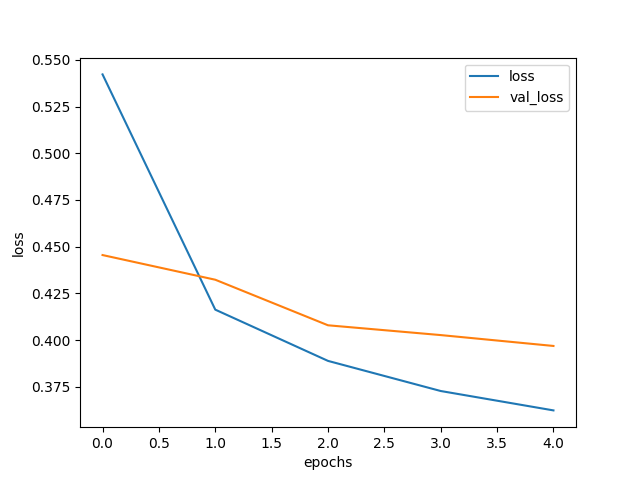
\includegraphics[scale=.35]{Loss_Exp9}
		\label{fig:LossExp9}
		\caption{Loss values of the finished 	project}
		\end{figure}
	\end{multicols}
\end{frame}
\subsection{Evaluation}
\begin{frame}{Evaluation}
	The purpose of these experiments is to determine if the parameters chosen for this project are optimal and, if not, correct them and know the reason behind the improvement.
	
	Lower loss and higher accuracy are preferred.
\end{frame}
\begin{frame}{Experiment Results}
	\begin{table}[!h]
	\caption{Experiment results}
	\vspace{0.2cm}
	\centering
	\begin{tabular}[t]{|l|l|l|l|l|}
	\hline
	\multicolumn{1}{|c|}{} & \multicolumn{2}{c|}{Training} & \multicolumn{2}{c|}{Cross-Validation}
	\\ \hline
	\ & Loss & Accuracy & Loss & Accuracy
	\\ \hline
	\hyperref[exp1]{Experiment 1} & 0.6916 & 0.7130 & \textbf{0.8709} & 0.6234
	\\ \hline
	\hyperref[exp2]{Experiment 2} & 0.5956 & 0.7576 & 0.7649 & 0.6821
	\\ \hline
	\hyperref[exp3]{Experiment 3} & 0.5829 & 0.7564 & 0.7373 & 0.6780
	\\ \hline
	\hyperref[exp4]{Experiment 4} & 0.5455 & 0.7741 & 0.6704 & 0.7110
	\\ \hline
	\hyperref[exp6]{Experiment 5} & 0.6222 & 0.6550 & 0.7186 & 0.5357
	\\ \hline
	\hyperref[exp7]{Experiment 6} & 0.6041 & 0.7451 & 0.6555 & 0.7097
	\\ \hline
	\hyperref[exp8]{Experiment 7} & 0.6030 & 0.7421 & 0.6579 & 0.7156
	\\ \hline
	\hyperref[exp9]{Experiment 8} & 0.3624 & 0.8337 & 0.3871 & \textbf{0.8124}
	\\ \hline
	\end{tabular}
\end{table}
\end{frame}

\section{Conclusions}

\begin{frame}{Conclusions}
	\begin{block}{Conclusion}
		In the end, the conclusion reached is that the hypothesis was correct; it is possible for a Machine Learning algorithm to predict how a person is feeling based on an input, albeit some faults can be caused by the datasets used in training it. This can be changed using some quality control on them, or using personalized data specifically catered to this project.
	\end{block}
	\begin{block}{Future Work}
		This project would greatly benefit from a dataset that takes into consideration sentences that can be said in any context and still be correctly classified. And, of course, the less ortographical errors there are, the better.
	\end{block}
\end{frame}


\begin{frame}{References}
	\centering
	\vspace*{-0.6cm}
	\setlength{\columnsep}{-0.2cm}
	\begin{multicols}{3}
		{\tiny \bibliography{biblio}}
	\end{multicols}
	
\end{frame}
\end{document}